\documentclass[a4paper,10pt, openright]{article}
\pagestyle{plain}
\usepackage{titlesec}
\titleformat{\chapter}[display]
{\normalfont\Large\bfseries}{\chaptertitlename\ \thechapter}{20pt}{\large}
\titleformat{\section}
{\normalfont\large\bfseries}{\thesection}{1em}{}
\usepackage[margin=0.45in]{geometry}
\usepackage[english]{babel} 
\usepackage{amssymb,amsmath,amsthm,amsfonts}
\usepackage{algorithm}
\usepackage{algpseudocode} 
\usepackage{graphicx, array}
\usepackage{xcolor}
\usepackage{float}
\usepackage{subfigure}
\usepackage{imakeidx}
\usepackage{tabularx}
\linespread{1.1}
\makeindex


\begin{document}
	\begin{center}
	{\Huge Topic Modeling and Sentiment Analysis for Amazon Book Reviews}\\
	{ Andres Bermeo Marinelli}\\
	{NLP Final Project, A.A. 2021-2022}
		
	\end{center}

\tableofcontents

\newpage
\section{Problem Statement \index{Problem Statement}}
The main aim of this project is to implement tools based on Natural Language Processing techniques to be used for the following tasks:

\begin{enumerate}
	\item Help publishers and authors understand the topics of books being sold on Amazon to have a better idea of the current interests and overall market situation.
	\item Classify user reviews in order to incorporate this knowledge in a collaborative based filtering technique where similar tastes between users are used to recommend new items.   
\end{enumerate}  

To address these problems, we perform topic modeling and sentiment analysis on a corpus of book summaries and corresponding amazon reviews.

After studying the most frequent words in the corpus of book descriptions, we extract the K main topics that characterize them by means of Latent Dirichlet Allocation (LDA), along with the 10 most relevant words for each topic. Consequently, we try to interpret the theme/meaning of each topic and analyze their association to the categories provided in the dataset. Lastly, by using the topic distribution of each document, we study how the popularity of each theme changes over time.

For sentiment analysis, we use RoBERTa to classify the reviews as positive or negative and compare them to grouped ground truth labels. Lastly, we fine-tune RoBERTa using HuggingFace's Trainer environment on our own data to improve the model. We compare this model to a baseline classifier which always predicts the most frequent class. 

\section{Data Description \index{Data Description}}
The dataset contains two separate files with data on books and their reviews. 

The first file contains details about $\sim 212,000$ books. In particular, it contains information such as title, author, published date, description, and category. Around $68,000$ ($30\%$) items have a missing description, so they are eliminated, since the main focus is to extract topics from the summaries of books. Furthermore, not all the books are in English. Since LDA implicitly assumes the same language for its probabilistic structure of document creation, we remove documents not in English after applying language recognition tools to the summaries. This leaves a total of $\sim 142,000$ items. In this subset, we study the frequency of the categories and find that the three most popular are fiction, history, and religion. However, the existing categories are $521$, so we limit ourselves to showing the top 10 most frequent.

\begin{figure}[H]
	\begin{center}
		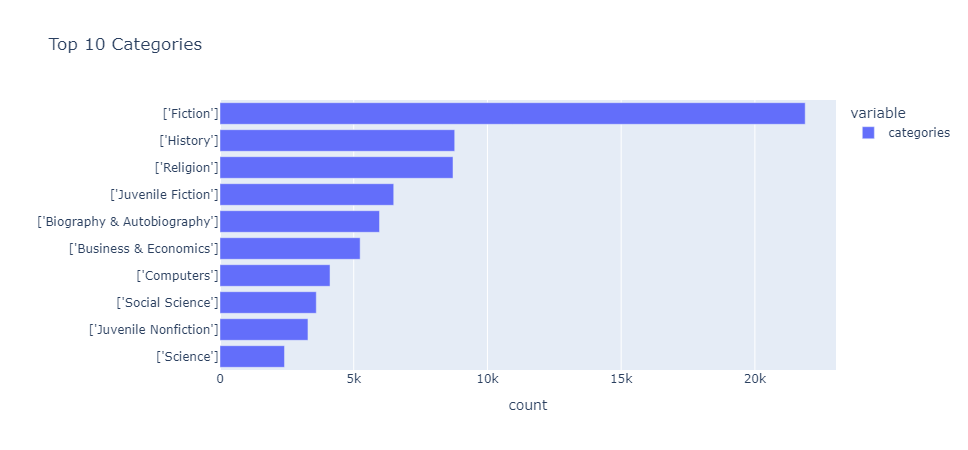
\includegraphics[width=20 cm, height=10 cm]{./Images/categories.png}
		\caption{The top 10 most frequent categories of books. "Fiction", "history", and "religion" figure among the top 3.}
		\label{fig:categories}
	\end{center}
\end{figure}
\newpage
The second file contains information about $3$ million reviews on the books contained in the first file. In particular, we have info such as book id (being reviewed), title of the book, id of user reviewing, summary of the review, text of the review, and finally a score from 1 to 5. The scores are severely imbalanced with 5 star reviews being the most predominant class.

\begin{figure}[H]
	\begin{center}
		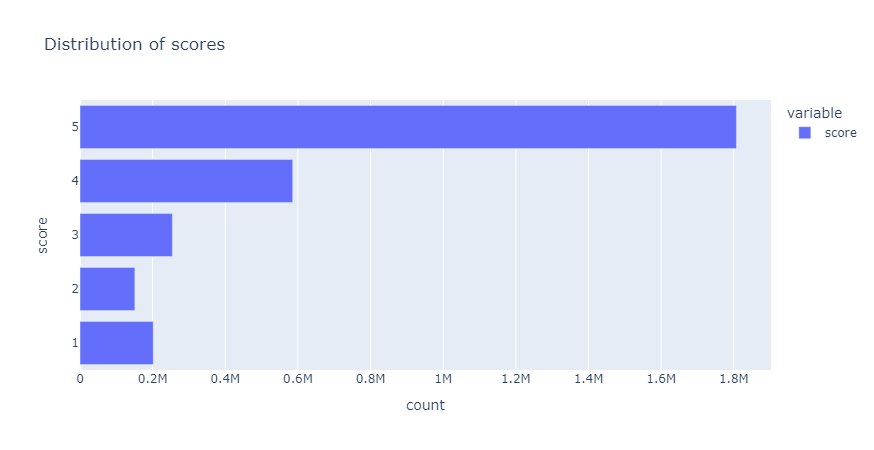
\includegraphics[width=18 cm, height=10 cm]{./Images/scores.png}
		\caption{The distribution of scores shows that classes are unbalanced and the majority is composed of 5 star reviews.}
		\label{fig:scores}
	\end{center}
\end{figure}

\section{Assessment and Performance Indexes \index{Assessment and Performance Indexes}}

With regard to parameter tuning, for topic modeling, LDA requires as input the number of topics $K$. To choose this value, we vary $K \in [2,...,20]$ and use two metrics: UMass and CV score\cite{firstbib}. The optimal number of topics is reached when these two scores are locally maximized. However, we also keep in mind the principle of Occam's razor which prefers simpler, more explainable models, sometimes at the expense of a lower metric/score. 

On the other hand, for sentiment analysis, we use accuracy, precision, recall, and f1 score. In particular, we used sklearn's classification report to quickly obtain a per-class score of the last three metrics as well as an overall accuracy of the model. In the end, when we compare the baseline with a fine-tuned instance of RoBERTa, we use balanced accuracy, micro, macro, and weighted f1 score. This is done to properly study the effects of class imbalance.

\section{Topic Modeling \index{Topic Modeling}}

After having eliminated items without book descriptions and non-English text, we are left with $\sim 142,000$ elements. At this point, to obtain an even more descriptive summary of the book, we concatenate the summary of the book with the title by separating these two with a period.

Then we aggressively pre-process the text to reduce variance to a minimum and capture the most meaning with the word descriptors after running LDA. In particular, we normalize the text by lower casing, removing all symbols and punctuation (except for hyphens and apostrophes); we tokenize using spacy, we keep the lemma of each word, we remove stop words contained in the default list of spacy, removing also words such as "book", "author", "write", and "story". Finally, we find the joint collocations with $PMI \ge 1.0$ and represent them as bi-grams. This final bound was chosen to limit the computational requirements and keep only the most meaningful collocations. 

We construct the word-cloud from the pre-processed descriptions to study the most frequent terms in order to have some prior ideas of some important topics/themes in the corpus. 

\begin{figure}[H]
	\begin{center}
		
\includegraphics[width=12 cm, height=9 cm]{./Images/wordcloud.png}
		\caption{The word-cloud of the most frequent terms in the corpus of book summaries. Terms such as "work", "world", "life", "history", "time", "love", "family" indicate the themes being discussed.}
		\label{fig:ldaword}
	\end{center}
\end{figure}

Some of the most frequent words such as "work", "world", "life", "history", "time", "love", "family", are very suggestive of the topics present in the corpus. These are powerful indicators of possible topics that we may find in the corpus. Also, we can see that they can be linked in some way to the most popular categories shown before. 

After having prepared the corpus for LDA, we must determine the number of topics to extract. To achieve this, we loop over $K \in [2,...,20]$ and train LDA on the first $10,0000$ documents, and compute UMass and CV scores on the next $40,000$. We set $\alpha = 0.01$ and $\eta =$ "auto". The former tells us to expect around one topic per document while the latter is related to the specificity of words to topics and enables LDA to learn a prior from the corpus. We obtain the following curves for varying $K$:

\begin{figure}[H]
	\begin{center}
		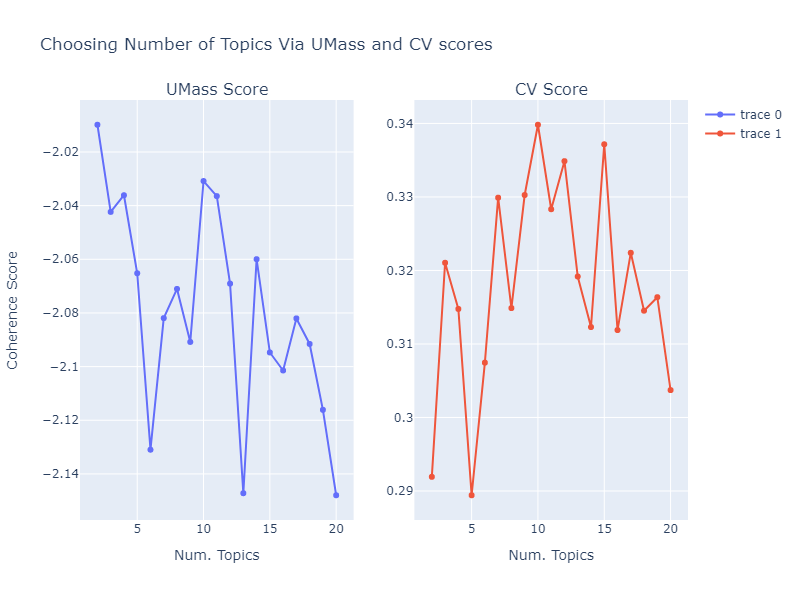
\includegraphics[width=16 cm, height=9 cm]{./Images/umasscvscore.png}
		\caption{UMass and CV scores with varying number of topics. The maximum occurs at $K=10$ which indicate the optimal number of topics.}
		\label{fig:umasscv}
	\end{center}
\end{figure}

As we can see, we obtain that the local maximum is at $K=10$ topics for both UMass and CV score. Specifically, for the CV score, $K=10$ represents a global maximum. 

Finally, we can extract the top 10 descriptors for each topics and examine the results.

\begin{table}[!ht]
	\centering
	\makebox[0cm]{\begin{tabular}{|l|l|l|l|l|l|l|l|l|l|l|}
		\hline
		~ & 	\texttt{Word 1}  & 	\texttt{Word 2} & 	\texttt{Word 3} &	\texttt{Word 4} & 	\texttt{Word 5} & 	\texttt{Word 6} & 	\texttt{Word 7} & 	\texttt{Word 8} & 	\texttt{Word 9} & 	\texttt{Word 10} \\ \hline
		\texttt{Topic 1} & recipe & food & guide & cookbook & cook & garden & plant & dish & cooking & eat \\ \hline
		\texttt{Topic 2} & child & life & god & love & parent & help & dog & little & animal & baby \\ \hline
		\texttt{Topic 3} & social & theory & political & study & history & science & economic & culture & human & american \\ \hline
		\texttt{Topic 4} & music & art & film & work & artist & original & include & guide & song & history \\ \hline
		\texttt{Topic 5} & bible & god & church & christian & jesus & testament & biblical & spiritual & study & christ \\ \hline
		\texttt{Topic 6} & student & guide & edition & provide & business & design & language & include & information & system \\ \hline
		\texttt{Topic 7} & love & novel & man & life & find & woman & murder & family & young & new \\ \hline
		\texttt{Topic 8} & game & baseball & sport & guide & player & bird & quilt & include & color & history \\ \hline
		\texttt{Topic 9} & poem & poetry & poet & litarature & work & american & history & publish & english & essay \\ \hline
		\texttt{Topic 10} & war & history & american & world & life & man & america & battle & year & new \\ \hline
	\end{tabular}}
\end{table}

As we can see, the topics are quite easy to interpret:
\begin{itemize}
	\item topic 1: \texttt{cooking}.
	\item topic 2: \texttt{family}.
	\item topic 3: \texttt{socio-economic science}.
	\item topic 4: \texttt{fine arts}.
	\item topic 5: \texttt{religion}.
	\item topic 6: \texttt{student help}.
	\item topic 7: \texttt{fictional romance}.
	\item topic 8: \texttt{sport \& outdoors}.
	\item topic 9: \texttt{poetry \& literature}.
	\item topic 10: \texttt{american history}.
\end{itemize}

\footnote{To differentiate between LDA topics and categories, we use bold font and italics, respectively.}We notice that \texttt{history} and \texttt{religion} reconnect exactly to the categories found in the top 10 list. Looking at the top 40 categories, we realize that a lot of the topics found by LDA are either explicitly contained as a category or represent a mix of these. For example, \texttt{cooking}, \texttt{family} figure by the same name in the 11th and 13th position respectively (actually, it's \textit{family \& relationships}). 

Other topics on the other hand, represent overlaps of categories. For example, \texttt{student help} is probably related to \textit{juvenile non-fiction} and \textit{self-help}; \texttt{socio-economic science} is an overlap of \textit{social science} and \textit{business \& economics}; \texttt{fine arts} is related to \textit{music}, \textit{art}, and \textit{performing arts}; \texttt{sport \& outdoors} is a mix of \textit{sport \& recreation}, \textit{health and fitness} and \textit{nature}; \texttt{fictional romance} is probably linked to \textit{fiction} and \textit{juvenile fiction}; finally, \texttt{poetry \& literature} is connected to \textit{poetry}, \textit{literary criticism}, and \textit{language arts \& disciplines}.

As we can see, the extracted topics are useful because they can help to summarize and group together the existing categories which are related. Furthermore, they can also condense information that in our case is given by analyzing $521$ categories.

Finally, we analyze how the topics change throughout the years. In particular, we will analyze the last 12 years (for graphical and practical reasons). We associate to each document the most relevant topic and plot how many items belong to each topic per year. Below we can see the results:


\begin{figure}[H]
	\begin{center}
		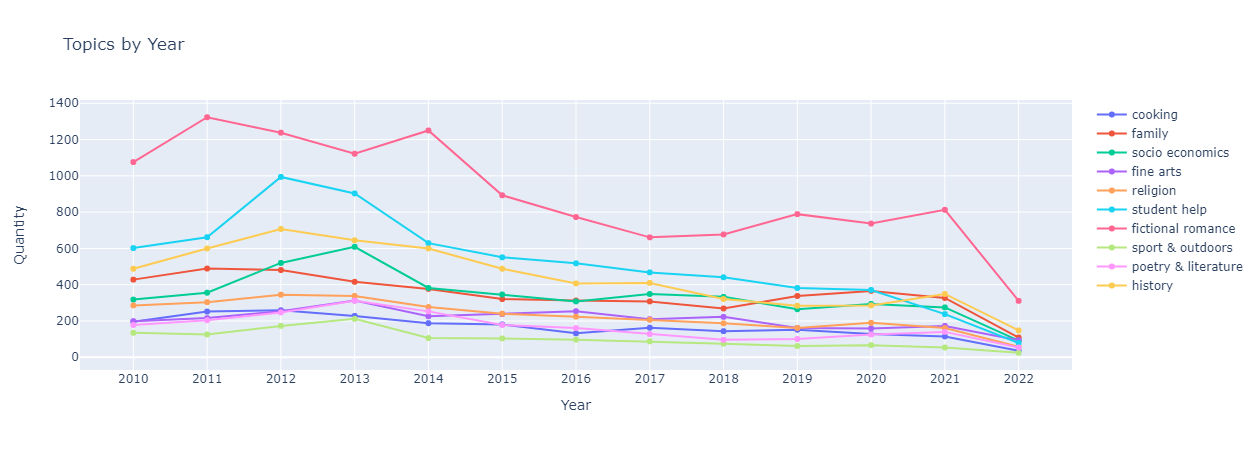
\includegraphics[width=16 cm, height=9 cm]{./Images/topicsbyyear.png}
		\caption{Frequency of topics per year since 2012. The overall trend is downwards, however, 2 years ago, \texttt{fictional romance} increased.}
		\label{fig:topicyears}
	\end{center}
\end{figure}


Some notable observations from the bar chart above:
\begin{enumerate}
\item In 2021, the number of books related to \texttt{fictional romance} and \texttt{family} has gone up. This could be due to the difficult times due to the pandemic which undoubtedly left lots of people with desires of affection and human contact\cite{secondbib} as well as an intriguing story to occupy their time during lockdown/quarantine. 
\item There was a noticeable increase in quantity of books related to \texttt{student help} in 2012. This could be linked to the boom in popularity of massive open online courses - MOOCs in those years\cite{thirdbib}. It could be that the boom in MOOCs cause an increase in the production of texts for helping students in various aspects.  
\item Not many books related to \texttt{sport \& outdoors} are produced. This could be due to the fact that this is a theme in which people prefer to learn by doing rather than reading. 
\item All the trends are decreasing and the sheer quantity of books are also less. This could be due to lack of data for these years or perhaps it could reflect a general trend of diminishing interest in books due to the internet. 
\end{enumerate}

\section{Sentiment Analysis \index{Sentiment Analysis}}


We have a dataset of 3 million reviews, with an associated score from 1 to 5 stars. We will focus on trying to predict the sentiment of a review based on the review summary instead of the entire text itself. This is done mainly for computational reasons. 

We try to create word clouds for positive and negative reviews, mainly to understand the type of sentiments we expect to find. One of the first difficulties is how to group 3 star reviews. In similar applications, it is customary to group 3 star reviews together with 4 and 5 stars and classify them as "positive". However, a quick sampling of 3 star reviews shows that they are associated to both negative and positive sentiments. Therefore, they were marked as "neutral", while 1-2 and 4-5 star reviews were classified as "negative" and "positive" respectively. 


\begin{figure}[H]
	\begin{center}
		\subfigure[]{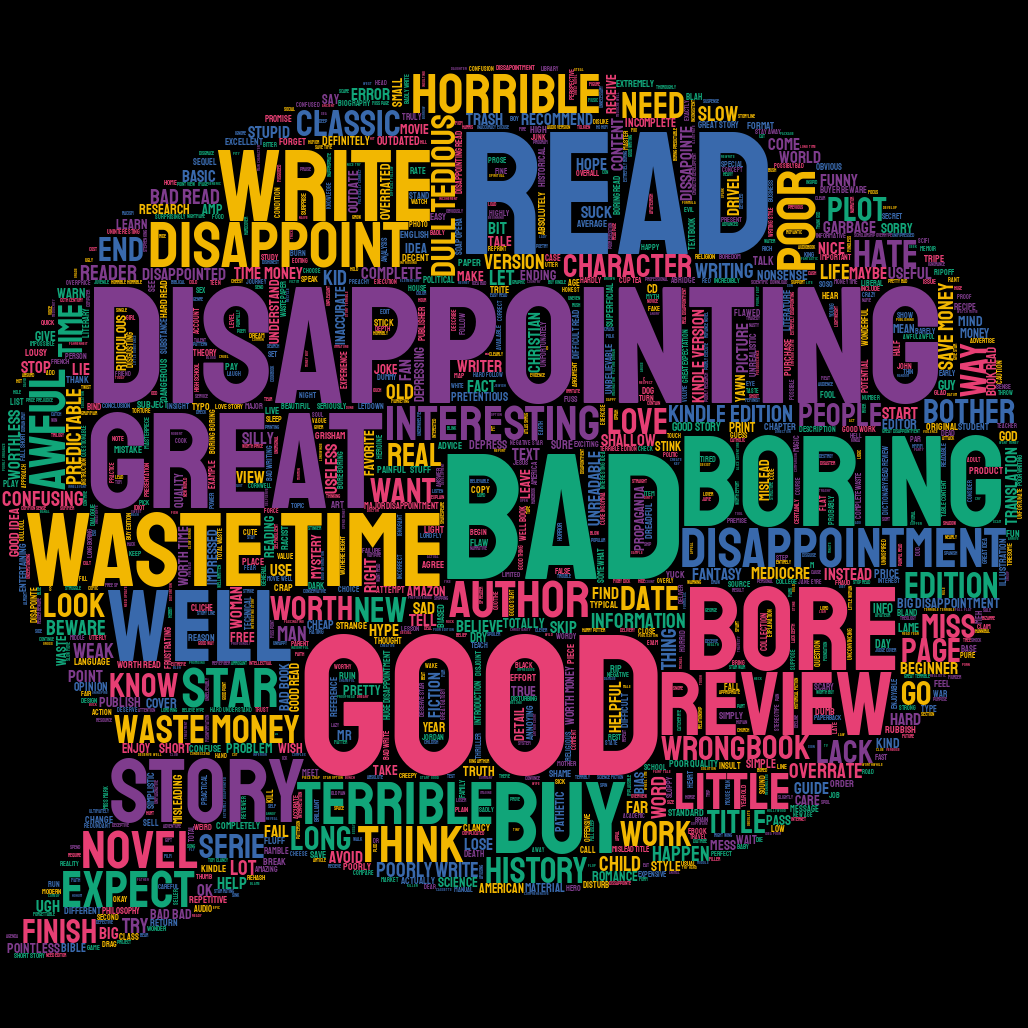
\includegraphics[width=9 cm, height=10 cm]{./Images/negative_wordcloud.png}}
		\subfigure[]{
\includegraphics[width=9 cm, height=10 cm]{./Images/positive_wordcloud.png}}
		\caption{Negative reviews word cloud (a) and positive reviews word cloud (b) reveal the words associated to negative and positive emotions respectively.}
		\label{fig:sentimentword}
	\end{center}
\end{figure}

For the negative sentiment word cloud (a) we have words such as "dissappointing", "bad", "boring", which indicate the emotions associated to these reviews. However, we also observe the presence of words such as "great" and "good", which seems counterintuitive at first glance. However, a quick search-and-find of the documents containing these terms shows that they are always preceded by "not" or "not so", in order to form a negative sentiment. This could have been avoided through the use of joint collocations.

For the positive sentiment word cloud (b), we see words such as "good", "great", "wonderful" and "excellent", which is a nice insight into the type of sentiments that are communicated with positive reviews. 

For the sentiment classification we use a pre-trained model from huggingface named "SiEBERT"\cite{fourthbib} which is an english language sentiment classifier. This model was trained on 15 different english datasets, including reviews and tweets and outputs a binary classification - positive or negative. The model has its own tokenizer which can be readily used. In fact, this is the reason that joint collocations were not included, since the tokenizer may separate the bigram automatically. 

Using the grouping described above, we remove all neutral reviews and fix a random subset of $100,000$ english reviews, to reduce computation time. Removing neutral reviews is an acceptable step since we are unable to classify them as positive or negative, and when studying the performance of the classifier, we need to be sure that the ground truth is correctly labeled, otherwise fine-tuning the model may lead to undesired behavior. 

We plot the distribution of the resulting dataset to verify that it still follows the original trend. As we can see it is still very unbalanced:


\begin{figure}[H]
	\begin{center}
		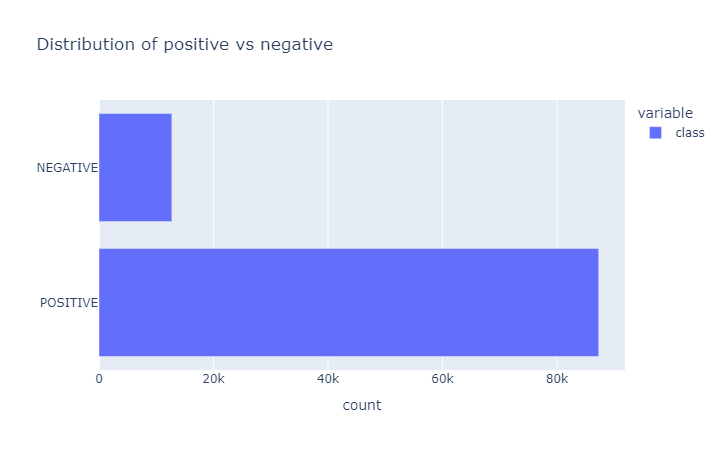
\includegraphics[width=18 cm, height=9 cm]{./Images/posvsneg.png}
		\caption{Distribution of positive and negative class.}
		\label{fig:posvsneg}
	\end{center}
\end{figure}

Using the model's tokenizer, we extract the predicted score for each review and run classification report on the results to obtain metrics per-class. 

\begin{table}[!ht]
	\centering
	\begin{tabular}{|l|l|l|l|l|}
		\hline
		RoBERTa & \texttt{precision} & \texttt{recall} & \texttt{f1-score} & \texttt{support} \\ \hline
		\texttt{negative} & 0.51 & 0.82 & 0.63 & 12720 \\ 
		\texttt{positive} & 0.97 & 0.89 & 0.93 & 87280 \\
		~ & ~ & ~ & ~ & ~ \\
		\texttt{accuracy} & ~ & ~ & 0.88 & 100000 \\ 
		\texttt{macro avg} & 0.74 & 0.85 & 0.78 & 100000 \\ 
		\texttt{weighted avg} & 0.91 & 0.88 & 0.89 & 100000 \\ \hline
	\end{tabular}
\end{table}

This model has high values of recall for both classes and a high precision for the positive class. However, it has a precision of $50\%$ for the negative class, which indicates that half of the time that the model classifies as negative, it is actually positive. This is largely due to the unbalance of the classes since the missing $10\%$ of the recall for the positive class corresponds to around $8,500$ documents which are positive but classified as negative. However, the size of this misclassification is comparable to the size of the negative class, which will cause its precision to go down.

We fine-tune this model to our dataset by using huggingface's trainer\cite{fifthbib} environment. We construct a train, validation, and test set by performing a random $60-20-20$ split. We set the learning rate $lr = 2e-5$, and train for $5$ epochs, evaluating and saving our model at each of these. We obtain the following results: 

\begin{figure}[H]
	\begin{center}
		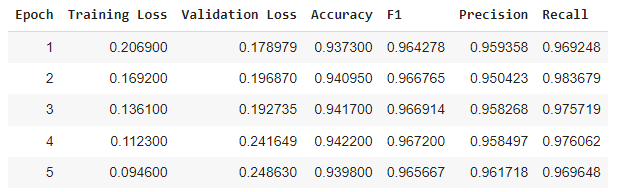
\includegraphics[width=16 cm, height=5 cm]{./Images/finetuning.png}
		\caption{Metrics for RoBERTa after fine-tuning on $60,000$ reviews. After the first 2 epochs, the model is clearly over-fitting as can be seen by the decrease in training loss and increase in validation loss.}
		\label{fig:robertaft}
	\end{center}
\end{figure}

After the 2nd epoch, the model is already over-fitting, as evidenced by the decrease in training loss and increase in validation loss. We use the model after the first epoch since this has the lowest validation loss. 

Running the classification again on the test set, we obtain the following classification report:

\begin{table}[!ht]
	\centering
	\begin{tabular}{|l|l|l|l|l|}
		\hline
		fine-tuned RoBERTa & \texttt{precision} & \texttt{recall} & \texttt{f1-score} & \texttt{support} \\ \hline
		\texttt{negative} & 0.77 \scriptsize ($\mathbf{+0.26}$) & 0.70 \scriptsize ($ \mathbf{-0.12}$) & 0.73 \scriptsize ($ \mathbf{+0.10}$) & 2561 \\ 
		\texttt{positive} & 0.96 \scriptsize ($ \mathbf{-0.01}$) & 0.97 \scriptsize ($ \mathbf{+0.08}$) & 0.96 \scriptsize ($ \mathbf{+0.03}$) & 17439 \\
		~ & ~ & ~ & ~ & ~ \\
		\texttt{accuracy} & ~ & ~ & 0.93 \scriptsize ($\mathbf{+0.05}$) & 20000 \\ 
		\texttt{macro avg} & 0.86    \scriptsize ($ \mathbf{+0.12}$) & 0.83 \scriptsize ($ \mathbf{-0.02}$) & 0.85 \scriptsize ($ \mathbf{+0.07}$) & 20000 \\ 
		\texttt{weighted avg} & 0.93 \scriptsize ($ \mathbf{+0.02}$) & 0.93 \scriptsize ($ \mathbf{+0.05}$) & 0.93 \scriptsize ($ \mathbf{+0.04}$) & 20000 \\ \hline
	\end{tabular}
\end{table}





As we can see, the model has noticeably improved compared to before. We have higher values for precision ($51\% \rightarrow 71\%$) and f1-score ($63\% \rightarrow 73\%$) for the negative class, and higher recall ($89\% \rightarrow 97\%$) and f1-score ($93\% \rightarrow 96\%$) for the positive class. Furthermore, the accuracy also increased ($88\% \rightarrow 93\%$ ). 

The precision for the positive class decreased slightly ($97\% \rightarrow 96\%$) and the recall dropped considerably ($82\% rightarrow 70\%$).

However, the performance metrics indicate an overall improvement and are more desirable for an all purpose application. 

We compare this model to a baseline classifier which predicts the most frequent class for all items. We show the final results below:

\begin{figure}[H]
	\begin{center}
		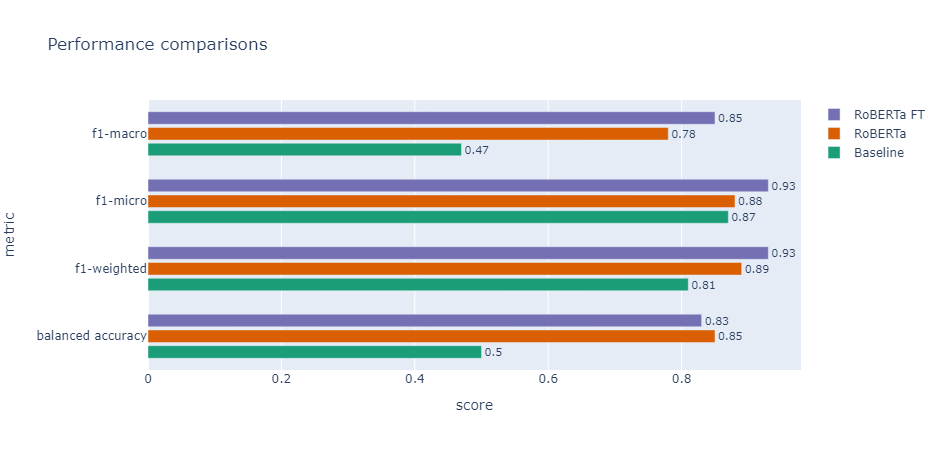
\includegraphics[width=18 cm, height=9 cm]{./Images/perfcomp.png}
		\caption{Comparison between baseline, RoBERTa, and RoBERTa fine-tuned. The latter model has the best overall performance.}
		\label{fig:perfcomp}
	\end{center}
\end{figure}

We notice that both the model and its fine-tuned version performs better than the baseline in all the metrics.

In particular, we see that the balanced accuracy for the baseline is reduced to $1/n_{classes}$ which is the accuracy of a random classifier. 

Both models also outperform the weighted and micro f1 scores, which is important due to the high imbalance of the classes. To briefly explain further, the baseline will correctly predict all the occurrences of the positive class, which account for approximately $85\%$ of the dataset. Thus, if we are weighting the metrics by their class weight, this will "hide" the null performance on the negative class. However, both models are able to outperform this and correctly predict the majority of the positive class but also $70\%$ of the negative class.

We are not surprised that the models outperform the baseline in f1-macro score since this gives equal weights to the classes and the baseline misclassifies all the negative instances. 

Lastly, the only area where the pre-trained model surpasses the fine-tuned model is in balanced accuracy. However, the difference is so small that it could be due to fluctuations in the testing set. In fact, we must remember that for the pre-trained model we compute the metrics on a test set which contained $100,000$ items, while the fine-tuned model only has $20,000$ reviews. A better approach would have been to fine-tune the model on $100,000$ items and then test it on another $100,000$ items. However, this was not done for computational reasons. 

\section{Results and Discussion \index{Results and Discussion}}

In the first section we extracted 10 topics from the corpus of book descriptions ( $\sim 200,000$ items) by maximizing UMass and CV scores. By analyzing the top 10 descriptors for each topic, we were able to draw connections to the categories of the dataset. In particular, we saw that all of the topics either appeared as a category, or encapsulated 2 or more categories which were very related. Furthermore, the topic descriptors also served to have a better idea of the type of words associated to each topic, which gives a deeper understanding of what a category means, rather than leaving it to interpretation. 

However, in the absence of supervision (i.e the categories), this tool could enable authors and publishing companies alike to obtain information about the topics of a corpus and study how their frequency changes over time. This in turn could give an insight into which categories are more popular and worth publishing or writing about. In our case, we saw that the topic of \texttt{fictional romance} was produced more frequently during the years of covid, which indicates perhaps, that this would've been a good moment to focus on this thematic. Another interesting observation was the increase in 2012 of books related to \texttt{student help} which coincided with the boom of MOOC's. Finally, the data showed an overall decline in volume, which could be due to lack of data collection or could indicate a general trend towards reading less. 

In the second section, we use a pre-trained RoBERTa classifier to predict reviews as positive or negative. The model was originally trained on 15 different datasets which made it much more versatile in terms ability to classify text accurately. After classifying a random sample of $100,000$ reviews, we observed that the model had a precision of $50\%$ for the negative class, which is the precision of a random classifier. 

Subsequently, the model was fine-tuned for $5$ epochs on a subset of $60,000$ reviews, and validated on $20,000$ items. After one epoch the model was at the optimal state compared to epochs later. Using the model weights obtained in the first epoch, we classified reviews on a held out test set of $20,000$ documents and found it outperformed the model without fine-tuning. 

Finally, we compared both models (with and without fine-tuning) to a baseline classifier which predicted the most frequent class. The fine-tuned model outperformed the other two in all of the aggregate metrics, such as f1-score weighted, micro, and macro. On the other hand, the balanced accuracy dropped slightly compared to the model without fine-tuning. 

This tool gives us a simple method to evaluate user reviews and integrate this knowledge into a recommender system which is based on user similarity. Specifically, if two users with similar features, rate the same items as positive and negative, then we could recommend items that one user liked to the other.

\newpage
\begin{thebibliography} {99}
	\bibitem{firstbib} https://www.os3.nl/\_media/2017-2018/courses/rp2/p76\_report.pdf
	\bibitem{secondbib} https://www.frontiersin.org/articles/10.3389/fpsyg.2021.798260/full
	\bibitem{thirdbib}	https://onlinelearninginsights.wordpress.com/2012/12/21/what-the-heck-happened-in-2012-review-of-the-top three-events-in-education/
	\bibitem{fourthbib} https://huggingface.co/siebert/sentiment-roberta-large-english?text=I+like+you.+I+love+you
	\bibitem{fifthbib}	https://huggingface.co/docs/transformers/training\#additional-resources
	
\end{thebibliography}
% to create index, uncomment line below. It has to be at end of doc to be generated automatically. 
% also note that the things I want indexed (the titles) are followed by \index{term i want indexed} and this DOES NOT show up. kind of like a tag)
%\printindex 
\end{document}